\documentclass[aspectratio=169, 10pt]{beamer}

% --- Theme & Styling ---
\usetheme{Madrid}
\usecolortheme{dolphin}
\usefonttheme{professionalfonts}

% Custom Colors
\definecolor{DeepBlue}{RGB}{28, 55, 99}
\definecolor{AccentBlue}{RGB}{43, 106, 177}
\definecolor{LightGray}{RGB}{245, 245, 245}
\definecolor{AlertRed}{RGB}{200, 40, 40}
\definecolor{PathGreen}{RGB}{34, 139, 34}
\definecolor{CodeGray}{RGB}{240, 240, 240}
\definecolor{Gold}{RGB}{218, 165, 32}

% Apply Colors
\setbeamercolor{structure}{fg=DeepBlue}
\setbeamercolor{frametitle}{bg=DeepBlue, fg=white}
\setbeamercolor{title}{bg=DeepBlue, fg=white}
\setbeamercolor{block title}{bg=AccentBlue, fg=white}
\setbeamercolor{block body}{bg=LightGray, fg=black}
\setbeamercolor{alerted text}{fg=AlertRed}

% --- Packages ---
\usepackage{tikz}
\usepackage{amsmath}
\usepackage{booktabs}
\usepackage{algorithm}
\usepackage{algpseudocode}
\usetikzlibrary{arrows.meta, positioning, calc, shapes, shadows, decorations.pathreplacing}

% --- Meta Data ---
\title[Unigram Implementation]{The SentencePiece Unigram Algorithm}
\subtitle{Implementation Reference \& Illustrative Examples}
\author{Gemini 3 \\{\tiny Prompted by: Shikhar Srivastava}}
\date{\today}

\begin{document}

% --- Title Slide ---
\begin{frame}
    \titlepage
\end{frame}

% --- Outline ---
\begin{frame}{Outline}
    \tableofcontents
\end{frame}

% ==========================================
% SECTION 1: OVERVIEW
% ==========================================
\section{1. The Unigram Blueprint}

\begin{frame}{1.1 Core Philosophy}
    Unlike BPE (bottom-up merge), Unigram is \textbf{top-down} and \textbf{probabilistic}.
    
    \begin{block}{The Independence Assumption}
        A sentence $X$ is a sequence of independent subwords.
        $$ P(S) = \prod_{i=1}^{M} P(x_i) $$
    \end{block}
    
    The true probability of sentence $X$ sums over \textit{all valid segmentations}:
    $$ P(X) = \sum_{S \in \text{valid}(X)} P(S) $$
    \textbf{Objective:} Maximize total log-likelihood $\mathcal{L} = \sum_{X \in \mathcal{D}} \log(P(X))$.
\end{frame}

\begin{frame}{1.2 The Algorithm Lifecycle}
    The Unigram model minimizes the vocabulary iteratively through this cycle:
    
    \vspace{0.3cm}
    \centering
    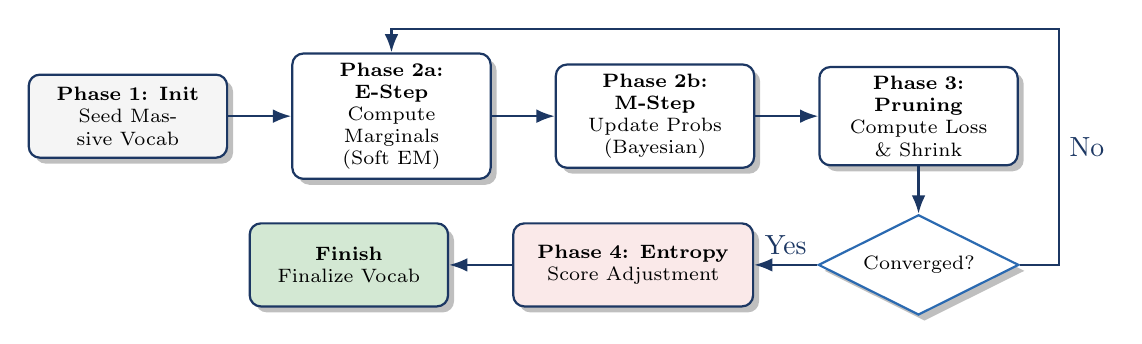
\begin{tikzpicture}[
        node distance=0.6cm and 0.8cm,
        auto,
        % Styles
        block/.style={rectangle, draw=DeepBlue, thick, fill=white, text width=6.5em, align=center, rounded corners, minimum height=3em, drop shadow, font=\scriptsize},
        decision/.style={diamond, draw=AccentBlue, thick, fill=white, text width=4em, align=center, aspect=2, drop shadow, font=\scriptsize},
        line/.style={draw, -Latex, thick, DeepBlue}
    ]
        % Nodes
        \node [block, fill=LightGray] (init) {\textbf{Phase 1: Init}\\Seed Massive Vocab};
        \node [block, right=of init] (estep) {\textbf{Phase 2a: E-Step}\\Compute Marginals\\(Soft EM)};
        \node [block, right=of estep] (mstep) {\textbf{Phase 2b: M-Step}\\Update Probs\\(Bayesian)};
        \node [block, right=of mstep] (prune) {\textbf{Phase 3: Pruning}\\Compute Loss \& Shrink};
        
        \node [decision, below=of prune] (check) {Converged?};
        
        \node [block, left=of check, fill=AlertRed!10, text width=8em] (entropy) {\textbf{Phase 4: Entropy}\\Score Adjustment};
        \node [block, fill=PathGreen!20, left=of entropy] (finish) {\textbf{Finish}\\Finalize Vocab};

        % Paths
        \path [line] (init) -- (estep);
        \path [line] (estep) -- (mstep);
        \path [line] (mstep) -- (prune);
        \path [line] (prune) -- (check);
        
        % Check Logic
        \path [line] (check) -- node [above] {Yes} (entropy);
        \path [line] (check.east) -- +(0.5,0) |- node [near start, right] {No} ($(estep.north)+(0,0.3)$) -- (estep.north);
        
        \path [line] (entropy) -- (finish);
    \end{tikzpicture}
\end{frame}

% ==========================================
% SECTION 2: INITIALIZATION
% ==========================================
\section{2. Phase 1: Initialization}

\begin{frame}{2.1 Phase 1: Seed Generation (Implementation)}
    Before EM starts, SentencePiece generates a ``Superset'' vocabulary. This step is critical for the top-down approach.
    
    \begin{enumerate}
        \item \textbf{Enhanced Suffix Array (ESA):} 
        The algorithm first computes the ESA of the entire training corpus. This allows for linear-time counting of all substrings.
        
        \item \textbf{Extraction:} 
        It extracts the most frequent substrings to form a massive seed vocabulary.
        \begin{itemize}
            \item \textit{Note:} This seed is much larger than the final target `vocab\_size` (e.g., if target is 32k, seed might start at 100k+).
        \end{itemize}
        
        \item \textbf{Initial Probabilities:} 
        $P(x)$ is typically initialized based on raw frequency counts in the corpus or uniformly.
    \end{enumerate}
\end{frame}

\begin{frame}{2.2 Phase 1 Example: The "Banana" Corpus}
    \textit{To visualize the seed generation (simplified without ESA):}
    
    \vspace{0.2cm}
    \textbf{Corpus:} $\mathcal{D} = \{ \text{``banana''} \}$
    
    \textbf{Step 1: Generate Seed Vocabulary}
    Extract frequent substrings from "banana".
    $$ V_{seed} = \{ \text{b, a, n, ba, na, ban, ana, nana} \} $$
    
    \textbf{Step 2: Initialize Probabilities}
    Assume Uniform Distribution for this example.
    $$ P(x) = \frac{1}{8} = 0.125 \quad \Rightarrow \quad \text{Cost} (-\log P) = 3.0 $$
\end{frame}

% ==========================================
% SECTION 3: THE EM LOOP
% ==========================================
\section{3. Phase 2: The EM Loop}

\begin{frame}{3.1 Phase 2a: The E-Step (Expectation)}
    \textbf{Goal:} Estimate the expected count of each subword given the current model parameters.
    
    \vspace{0.2cm}
    \begin{columns}[T]
        \begin{column}{0.48\textwidth}
            \begin{block}{Soft EM (Actual Implementation)}
                SentencePiece uses the \textbf{Forward-Backward Algorithm} to compute marginal probabilities.
                $$ E[x] = \sum_{S \in \text{valid}(X)} P(S|X) \cdot \text{count}(x, S) $$
                This sums probability mass over \textit{all} possible segmentations, not just the best one.
            \end{block}
        \end{column}
        
        \begin{column}{0.48\textwidth}
            \begin{alertblock}{Contrast with Hard EM}
                Hard EM (Viterbi) considers only the single best path.
                \begin{itemize}
                    \item Used in Phase 3 (Pruning) for speed.
                    \item \textbf{Not} used in Phase 2a (Training) by default.
                \end{itemize}
            \end{alertblock}
        \end{column}
    \end{columns}
\end{frame}

\begin{frame}{3.2 Visualization: Building the Lattice}
    Segmenting ``banana''. Edges are subwords; Cost is 3.0 per edge.
    
    \vspace{0.3cm}
    \centering
    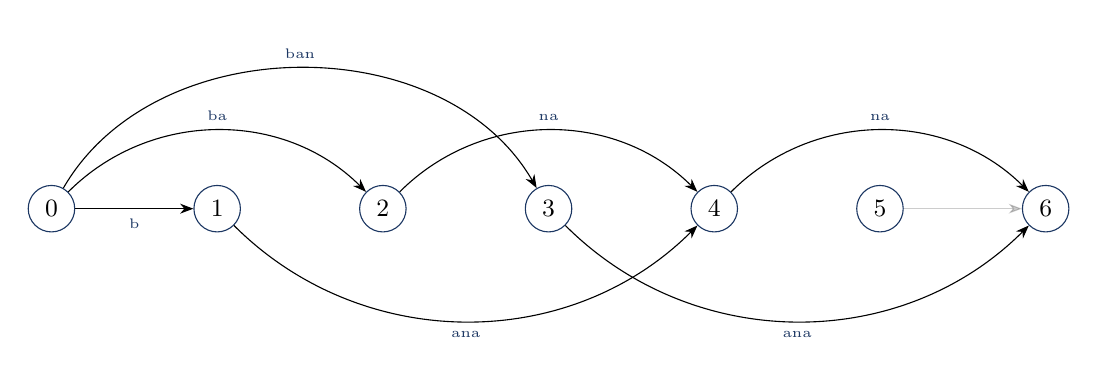
\begin{tikzpicture}[
        node distance=1.5cm,
        >=Stealth,
        state/.style={circle, draw=DeepBlue, fill=white, minimum size=0.5cm, font=\small},
        edge_label/.style={midway, above, font=\tiny, text=DeepBlue}
    ]
        \node[state] (0) {0};
        \node[state, right=of 0] (1) {1};
        \node[state, right=of 1] (2) {2};
        \node[state, right=of 2] (3) {3};
        \node[state, right=of 3] (4) {4};
        \node[state, right=of 4] (5) {5};
        \node[state, right=of 5] (6) {6};
        
        % Edges
        \draw[->] (0) -- node[edge_label, below] {b} (1);
        \draw[->] (0) to[bend left=45] node[edge_label] {ba} (2);
        \draw[->] (0) to[bend left=60] node[edge_label] {ban} (3);
        \draw[->] (2) to[bend left=45] node[edge_label] {na} (4);
        \draw[->] (4) to[bend left=45] node[edge_label] {na} (6);
        \draw[->] (1) to[bend right=45] node[edge_label, below] {ana} (4);
        \draw[->] (3) to[bend right=45] node[edge_label, below] {ana} (6);
        \draw[->, opacity=0.2] (5) -- (6); % Filler
    \end{tikzpicture}
\end{frame}

\begin{frame}{3.3 Visualization: The Viterbi Winner}
    If we used Hard EM (Viterbi), we would select the path with the \textbf{Lowest Total Cost}.
    
    \begin{enumerate}
        \item $b+a+n+a+n+a$ (6 tokens) $\to$ Cost $18$
        \item $ba+na+na$ (3 tokens) $\to$ Cost $9$
        \item $ban+ana$ (2 tokens) $\to$ Cost $6$ \textcolor{PathGreen}{\textbf{(Winner)}}
    \end{enumerate}
    
    \begin{block}{Insight}
        Since initial costs are uniform, Viterbi effectively selects the path with the \textbf{fewest tokens}. This is why ``ban'' + ``ana'' beats the others.
    \end{block}
\end{frame}

\begin{frame}{3.4 Phase 2b: The M-Step (Maximization)}
    \textbf{Goal:} Update probabilities based on E-Step expected counts.
    
    \begin{block}{Standard Expectation Maximization}
        $$ P_{new}(x) = \frac{\text{expected\_count}(x)}{\text{total\_observed\_tokens}} $$
    \end{block}
    
    \begin{alertblock}{Implementation Detail: Bayesian Estimation}
        SentencePiece actually uses a \textbf{Bayesian approach} (Dirichlet prior) to handle sparsity:
        
        $$ \theta_{new} \propto \exp(\Psi(C_{expected}) - \Psi(C_{total})) $$
        
        \small \textit{*Where $\Psi$ is the Digamma function (lines 393-395). This acts as a sparse prior, smoothing the distribution.}
    \end{alertblock}
\end{frame}

% ==========================================
% SECTION 4: PRUNING (DETAILED)
% ==========================================
\section{4. Phase 3: Pruning (Detailed Implementation)}

\begin{frame}{4.1 The Pruning Logic: Overview}
    The Pruning Step determines which tokens are "redundant".
    
    \vspace{0.2cm}
    \textbf{Key Implementation Details (File: \texttt{unigram\_model\_trainer.cc}):}
    \begin{enumerate}
        \item \textbf{Hard EM Switch:} Unlike training (Soft EM), pruning uses \textbf{Viterbi} (Best Path) counts to estimate token frequency (lines 452).
        \item \textbf{Second Best Path Strategy:} To calculate "Loss", it explicitly finds the 2-best segmentations for every token (lines 418).
        \item \textbf{Descending Sort:} It sorts candidates by Loss (Descending) and keeps the top \% (lines 519).
    \end{enumerate}
\end{frame}

\begin{frame}{4.2 Step 1: Self-Segmentation (The "Always Keep" Logic)}
    Before calculating loss, we check if the token is even useful to represent \textit{itself}.
    
    \begin{algorithmic}[1]
        \For{each token $t$ in vocab}
            \State Run \texttt{lattice.NBest(2)} on string "$t$"
            \If{Best Path splits $t$ (size $\ge$ 2)}
                \State \texttt{always\_keep[t] = false} \Comment{Prune immediately}
                \State \textit{Ex: "ABCD" $\to$ "AB" + "CD" is better than "ABCD"}
            \ElsIf{No 2nd Best Path exists}
                \State \texttt{always\_keep[t] = true} \Comment{Keep (Essential)}
            \Else
                \State Store 2nd Best Path in \texttt{alternatives[t]}
            \EndIf
        \EndFor
    \end{algorithmic}
\end{frame}

\begin{frame}{4.3 Step 2: The Loss Approximation}
    $$ \text{Loss}_t = \mathcal{L}_{total} - \mathcal{L}_{\text{without } t} $$
    
    We approximate $\mathcal{L}_{without\_t}$ by forcing the Viterbi path to take the "Second Best" route whenever it encounters token $t$.
    
    \vspace{0.3cm}
    \textbf{Intuition:}
    \begin{itemize}
        \item If $t$ is frequently used in the corpus, removing it forces many detours.
        \item If the "detour" (alternative) is much more expensive (lower prob), the Loss is high.
        \item If the detour is cheap (similar prob), the Loss is low.
    \end{itemize}
\end{frame}

\begin{frame}{4.4 Exact Loss Formula (Code Analysis)}
    \textbf{Code:} \texttt{unigram\_model\_trainer.cc} lines 490-506
    
    $$ L_t = F_t \times (\log P(t) - \log P_{\text{alt}}) $$
    
    \textbf{The "Denominator Shift" Detail:}
    When replacing token $t$ with a sequence of alternatives (e.g., $t \to a+b$), the total token count of the corpus increases. The code explicitly adjusts the log-sum for normalization:
    
    $$ \Sigma_{new} = \Sigma_{old} + \text{freq}[t] \times (\text{len}(\text{alt}) - 1) $$
    
    This ensures the "Alternative Probability" $P_{\text{alt}}$ is calculated against the correct theoretical vocabulary volume.
\end{frame}

\begin{frame}{4.5 Example: Loss Calculation for "ana"}
    \textbf{Scenario:} "ana" appears once. Total Corpus Cost: -1.38.
    
    \textbf{1. With "ana":} Path is "ban"+"ana". LogProb = -1.38.
    
    \textbf{2. Without "ana":} Alternative is "ba"+"na"+"na".
    \begin{itemize}
        \item Alternative consists of 3 tokens (vs 1).
        \item Cost dramatically increases to -12.0.
    \end{itemize}

    \textbf{Calculation:}
    $$ \text{Loss} = \underbrace{1.0}_{\text{Freq}} \times (\underbrace{-1.38}_{\text{Current}} - \underbrace{-12.0}_{\text{Alt}}) = \textbf{10.62} $$
    
    \textbf{Decision:} High Loss $\to$ Keep.
\end{frame}

% ==========================================
% SECTION 5: MODIFICATION
% ==========================================
\section{5. The Rényi Entropy Modification}

\begin{frame}{5.1 The New Objective}
    Standard Unigram optimizes strictly for Likelihood. We want to target a specific \textbf{Rényi Entropy ($\alpha$)}:
    
    $$ H_\alpha(P) = \frac{1}{1-\alpha} \log \left( \sum_{x \in V} p(x)^\alpha \right) $$
    
    \begin{alertblock}{Implementation Strategy: Phase 4}
        This modification happens \textbf{after the standard EM loop finishes} (Line 746).
        It is a post-processing score adjustment step using \textbf{Empirical Frequencies}.
    \end{alertblock}
\end{frame}

\begin{frame}{5.2 Limits of Rényi Efficiency for Unigram}
    \centering
    \textbf{The Landscape of Tokenization Entropy ($V$ = Fixed Vocabulary Size)}
    
    \vspace{0.5cm}
    
    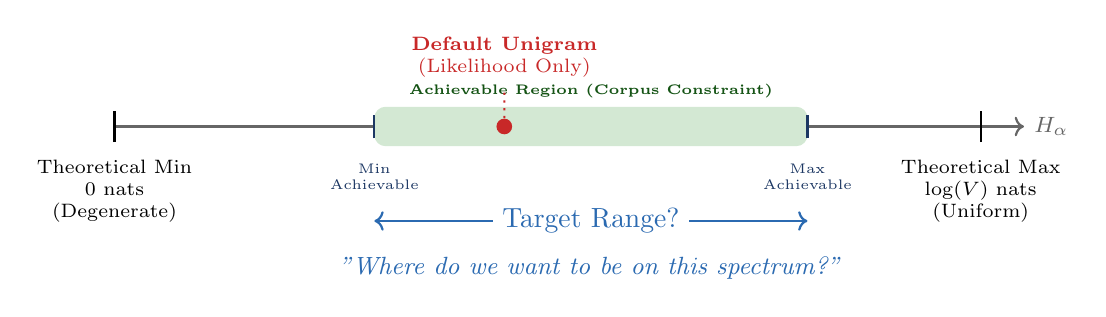
\begin{tikzpicture}[xscale=1.1, yscale=1]
        % --- Styles ---
        \tikzstyle{marker}=[circle, fill=DeepBlue, inner sep=2pt]
        \tikzstyle{labelnode}=[font=\scriptsize, align=center]
        
        % --- 1. Theoretical Axis ---
        \draw[->, thick, black!60] (0,0) -- (10.5,0) node[right] {\footnotesize $H_\alpha$};
        
        % Theoretical Min/Max Labels
        \draw[thick] (0, -0.2) -- (0, 0.2);
        \node[labelnode, below=0.3cm] at (0,0) {Theoretical Min\\$0$ nats\\(Degenerate)};
        
        \draw[thick] (10, -0.2) -- (10, 0.2);
        \node[labelnode, below=0.3cm] at (10,0) {Theoretical Max\\$\log(V)$ nats\\(Uniform)};
        
        % --- 2. Achievable Region (The "Zipf Barrier") ---
        % Natural language cannot be perfectly uniform due to grammar/Zipf's law
        \fill[PathGreen!20, rounded corners] (3, -0.25) rectangle (8, 0.25);
        \node[font=\tiny, text=PathGreen!60!black] at (5.5, 0.45) {\textbf{Achievable Region (Corpus Constraint)}};
        
        % --- 3. Points of Interest ---
        
        % Standard Unigram
        \node[marker, fill=AlertRed] (std) at (4.5, 0) {};
        \node[labelnode, text=AlertRed, above=0.5cm] (std_label) at (4.5,0) {\textbf{Default Unigram}\\(Likelihood Only)};
        \draw[dotted, thick, AlertRed] (std) -- (std_label);
        
        % Min Achievable
        \draw[thick, DeepBlue] (3, -0.15) -- (3, 0.15);
        \node[labelnode, below=0.1cm, font=\tiny, text=DeepBlue] at (3,-0.25) {Min\\Achievable};
        
        % Max Achievable
        \draw[thick, DeepBlue] (8, -0.15) -- (8, 0.15);
        \node[labelnode, below=0.1cm, font=\tiny, text=DeepBlue] at (8,-0.25) {Max\\Achievable};
        
        % --- 4. The Target Question ---
        \draw[<->, thick, AccentBlue] (3, -1.2) -- (8, -1.2) node[midway, fill=white, text=AccentBlue] {Target Range?};
        \node[font=\small, text=AccentBlue, align=center] at (5.5, -1.8) {\textit{"Where do we want to be on this spectrum?"}};
        
    \end{tikzpicture}
\end{frame}

\begin{frame}{5.3 Achieving the Target Range}
    \begin{columns}[T]
        \begin{column}{0.5\textwidth}
            \begin{block}{The Challenge}
                \begin{itemize}
                    \item \textbf{Theoretical Max} is unreachable because language follows a Power Law (Zipf).
                    \item \textbf{Default Unigram} naturally clusters near the lower end to minimize encoded length.
                \end{itemize}
            \end{block}
        \end{column}
        
        \begin{column}{0.48\textwidth}
            \begin{alertblock}{The Strategy (Hint)}
                To move the needle along the spectrum:
                \vspace{0.2cm}
                
                \textbf{1. To Increase Entropy ($\to$):} 
                Penalize frequent tokens, forcing the model to use a wider variety of pieces.
                
                \vspace{0.2cm}
                \textbf{2. To Decrease Entropy ($\leftarrow$):}
                Reward frequent tokens, concentrating mass on a smaller core vocabulary.
            \end{alertblock}
        \end{column}
    \end{columns}
    
    \vspace{0.5cm}
    \centering
    \textit{We achieve this by iteratively adjusting piece scores ($P_{model}$) \\ until the measured Empirical Entropy matches the target.}
\end{frame}

\begin{frame}{5.4 Why Empirical Frequencies?}
    The code intentionally ignores the model's internal probability parameters ($P_{model}$) and instead measures the \textbf{actual usage} of tokens ($P_{empirical}$) via Viterbi.
    
    \vspace{0.3cm}
    \textbf{Reasoning:}
    \begin{itemize}
        \item Adjusting model scores changes the Viterbi path.
        \item We want the \textit{final segmentation} to have the desired entropy, not just the abstract model parameters.
        \item This creates a feedback loop: Adjust Score $\to$ Run Viterbi $\to$ Measure Entropy $\to$ Adjust Score.
    \end{itemize}
\end{frame}

\begin{frame}[fragile]{5.5 The Adjustment Algorithm (Gradient-like)}
    \textbf{File:} \texttt{src/unigram\_model\_trainer.cc} :: \texttt{OptimizeEntropyViaScoreAdjustment}
    
    We shift token scores based on their deviation from the Mean Frequency ($\mu$).
    
    \begin{algorithmic}[1]
        \State Compute $H_{curr}$ using \textbf{Empirical Frequencies}
        \If{$H_{curr} < H_{target}$} \Comment{Need MORE Entropy (Uniformity)}
             \For{$i \leftarrow 0$ to $|V|$}
                \State \texttt{score[i] += learning\_rate * (mean\_freq - freq[i])}
                \State \Comment{Boosts Rare tokens (freq < mean)}
            \EndFor
        \Else \Comment{Need LESS Entropy (Spikiness)}
            \For{$i \leftarrow 0$ to $|V|$}
                \State \texttt{score[i] += learning\_rate * (freq[i] - mean\_freq)}
                \State \Comment{Boosts Common tokens (freq > mean)}
            \EndFor
        \EndIf
    \end{algorithmic}
\end{frame}

\begin{frame}
    \centering
    \Huge \textcolor{DeepBlue}{Thank You}
    
    \vspace{0.5cm}
    \normalsize
    \textit{Questions?}
\end{frame}

\end{document}

